\chapter{Resultados e Discussão}

\section{Rede de Sensores Sem Fio}
Nesta seção serão apresentados os resultados parciais obtidos no desenvolvimento da Rede de Sensores sem fio.

\subsection{Testes utilizando a IDE Arduino}
Inicialmente foram efetuados testes utilizando o módulo NodeMCU sendo programado utilizando-se a IDE do Arduino. Para efetuar a leitura do sensor de temperatura e umidade do ar de uma forma mais simples foi utilizado a biblioteca DHT.h. Como resultado foram obtidos alguns códigos, apresentados nos Quadros \ref{tab:funcao-temperatura}, \ref{tab:funcao-umidade} e \ref{tab:funcao-request}:

\begin{quadro}[H]
\centering
\caption{Função que lê a temperatura do sensor.}
\vspace{-\baselineskip}
\begin{minted}[
frame=single,
framesep=2mm,
baselinestretch=1.2,
bgcolor=LightGray,
fontsize=\footnotesize,
% linenos
]{c++}

float getTemperature() {
    float temp = dht.readTemperature();
    
    if (isnan(temp)) {
        Serial.println("Failed to read from DHT sensor!");
        return;
    }
    
    return temp;
}
\end{minted}
\vspace{-1.2cm}
\label{tab:funcao-temperatura}
\fonte{Do Autor (2018).}
\end{quadro}

O Quadro \ref{tab:funcao-temperatura} mostra uma função que é responsável por efetuar a coleta de temperatura pelo sensor DHT11, essa temperatura pode ser coletada em Celsius ou em Fahrenheit, neste caso iremos utilizar apenas o valor em celsius.

\begin{quadro}[H]
\centering
\caption{Função que lê a umidade do sensor.}
\vspace{-\baselineskip}
\begin{minted}[
frame=single,
framesep=2mm,
baselinestretch=1.2,
bgcolor=LightGray,
fontsize=\footnotesize,
% linenos
]{c++}

float getHumidity() {
    float hum = dht.readHumidity();
    
    if (isnan(hum)) {
        Serial.println("Failed to read from DHT sensor!");
        return;
    }
    
    return hum;
}
\end{minted}
\vspace{-1.2cm}
\label{tab:funcao-umidade}
\fonte{Do Autor (2018).}
\end{quadro}

Já no Quadro \ref{tab:funcao-umidade} temos o a função que é responsável por efetuar a coleta de umidade do ar pelo sensor DHT11. O valor é coletado em porcentagem.

\begin{quadro}[H]
\centering
\caption{Função que envia um objeto JSON com os valores medidos.}
\vspace{-\baselineskip}
\begin{minted}[
frame=single,
framesep=2mm,
baselinestretch=1.2,
bgcolor=LightGray,
fontsize=\footnotesize,
% linenos
]{c++}

void sendRequest(WiFiClient client) {
  StaticJsonBuffer<400> jsonBuffer;

  JsonObject& data = jsonBuffer.createObject();

  data["humidity"] = getHumidity();
  data["temperature"] = getTemperature();

  client.println(String("POST ") + url + " HTTP/1.1");
  client.println(String("Host: ") + host);
  client.println("Cache-Control: no-cache");
  client.println("Content-Type: application/json");
  client.print("Content-Length: ");
  client.println(data.measurePrettyLength());

  client.println();

  data.prettyPrintTo(client);
}
\end{minted}
\vspace{-1.2cm}
\label{tab:funcao-request}
\fonte{Do Autor (2018).}
\end{quadro}

Esta função (Quadro \ref{tab:funcao-request}) monta um objeto JSON contendo os valores obtidos pelo sensor de temperatura e umidade do ar DHT11. Após montar este objeto é feito uma requisição do tipo POST na aplicação Web onde será armazenado em um banco de dados.

\subsection{Desenvolvimento utilizando MicroPython}

Depois de realizados estes testes utilizando a IDE do Arduino, foi instalado o \textit{firmware} MicroPython que possibilita que o módulo NodeMCU seja programado utilizando-se a linguagem de Programação Python.

A programação foi realizada da seguinte forma, o nó se conecta a uma rede \textit{wifi} (Quadro \ref{tab:funcao-conecta}) e, após estar conectado, faz a coleta de dados de todos os sensores ligados a ele (Quadro \ref{tab:funcao-coleta}). Após coletar os dados, eles são publicados no broker mqtt (Quadro \ref{tab:funcao-publica}), feito isso, o nó entra em modo \textit{sleep}. Este ciclo irá se repetir constantemente, sendo que o nó será acordado apos um intervalo de tempo pré definido.

\begin{quadro}[H]
\centering
\caption{Função que conecta o nó a uma rede wifi.}
\vspace{-\baselineskip}
\begin{minted}[
frame=single,
framesep=2mm,
baselinestretch=1.2,
bgcolor=LightGray,
fontsize=\footnotesize,
% linenos
]{python}

def do_connect():
    networks = list(wifi.scan())
    for net in networks:
        if (net[0].startswith('AP_IFSUL') 
            or net[0].startswith('IF-CampusMuz')) 
            and net[4] == 0:
            
            wifi.connect(str(net[0].decode()), '')

            for t in range(0, 120):
                if wifi.isconnected():
                    return True

                time.sleep_ms(400)

            return None

\end{minted}
\vspace{-1.2cm}
\label{tab:funcao-conecta}
\fonte{Do Autor (2018).}
\end{quadro}

\begin{quadro}[H]
\centering
\caption{Função que coleta os dados dos sensores.}
\vspace{-\baselineskip}
\begin{minted}[
frame=single,
framesep=2mm,
baselinestretch=1.2,
bgcolor=LightGray,
fontsize=\footnotesize,
% linenos
]{python}

def get_sensors_data(self):

    dhtSensor = DHTSensor(
        vcc=self.conf['dht']['vcc'], 
        signal=self.conf['dht']['signal']
    )
    
    leafWetnessSensor = LeafWetnessSensor(
        vcc=self.conf['leafWetness']['vcc'],
        signal=self.conf['leafWetness']['signal']
    )
        
    tick = time.ticks_ms()
    while True:
        delta = time.ticks_diff(time.ticks_ms(), tick)
        if delta > (200):
            break

    dhtValues = dhtSensor.get_value()
    leafWetnessValue = leafWetnessSensor.get_value()

    data = {
        'humidity': dhtValues['humidity'],
        'temperature': dhtValues['temperature'],
        'leafWetness': leafWetnessValue
    }

    dhtSensor.__del__()
    leafWetnessSensor.__del__()

\end{minted}
\vspace{-1.2cm}
\label{tab:funcao-coleta}
\fonte{Do Autor (2018).}
\end{quadro}

\begin{quadro}[H]
\centering
\caption{Função que publica os dados.}
\vspace{-\baselineskip}
\begin{minted}[
frame=single,
framesep=2mm,
baselinestretch=1.2,
bgcolor=LightGray,
fontsize=\footnotesize,
% linenos
]{python}

def send_data(self):
    id = 'esp8266_' + ubinascii.hexlify(machine.unique_id()).decode()
    HOST = self.conf['mqtt']['host']
    PORT = self.conf['mqtt']['port']
    USER = self.conf['mqtt']['user']
    PASS = self.conf['mqtt']['pass']
    topic = self.conf['mqtt']['topic']

    node = self.get_node_information()
    sensors = self.get_sensors_data()

    data = { 'node': node, 'sensors': sensors }

    mqtt_client = MQTTClient(id, HOST, PORT, USER, PASS)
    
    try:
        mqtt_client.connect()

        mqtt_client.publish(topic, json.dumps(data))

        while True:
            data = self.get_saved_data()

            if data is not None:
                mqtt_client.publish(topic, json.dumps(data))
            else:
                break
        
        mqtt_client.disconnect()

    except:            
        if not self.save_data(data):
            machine.reset()

\end{minted}
\vspace{-1.2cm}
\label{tab:funcao-publica}
\fonte{Do Autor (2018).}
\end{quadro}

\subsection{Montagem dos Nós}
A montagem dos nós foi feita utilizando \textit{protoboard}, que são placas para experimentação onde não é necessário soldar os componentes do circuito. Os componentes foram conectados seguindo o esquema mostrado na Figura \ref{fig:no-publicador}.

Na Figura \ref{fig:no-interno}, podemos ver os componentes dispostos dentro de uma caixa de pvc impermeável, onde eles serão encapsulados. A caixa foi vedada com silicone para evitar que os componentes tenham contato com a água que aspergida pelo sistema de nebulização. 

\begin{figure}[H]
    \centering
    \includegraphics[scale=0.1]{04-figuras/no-interior.jpg}
    \caption{Parte interna de um nó publicador.}
    \vspace{-\baselineskip}
    \fonte{Do Autor (2018).}
    \label{fig:no-interno}
\end{figure}

Já na Figura \ref{fig:no-externo2} temos o nó já encapsulado, podemos ver o painel solar que foi posicionado no topo da caixa e os sensores de umidade relativa do ar, temperatura e molhamento foliar que estão ligados ao controlador por meio de fios.

\begin{figure}[H]
    \centering
    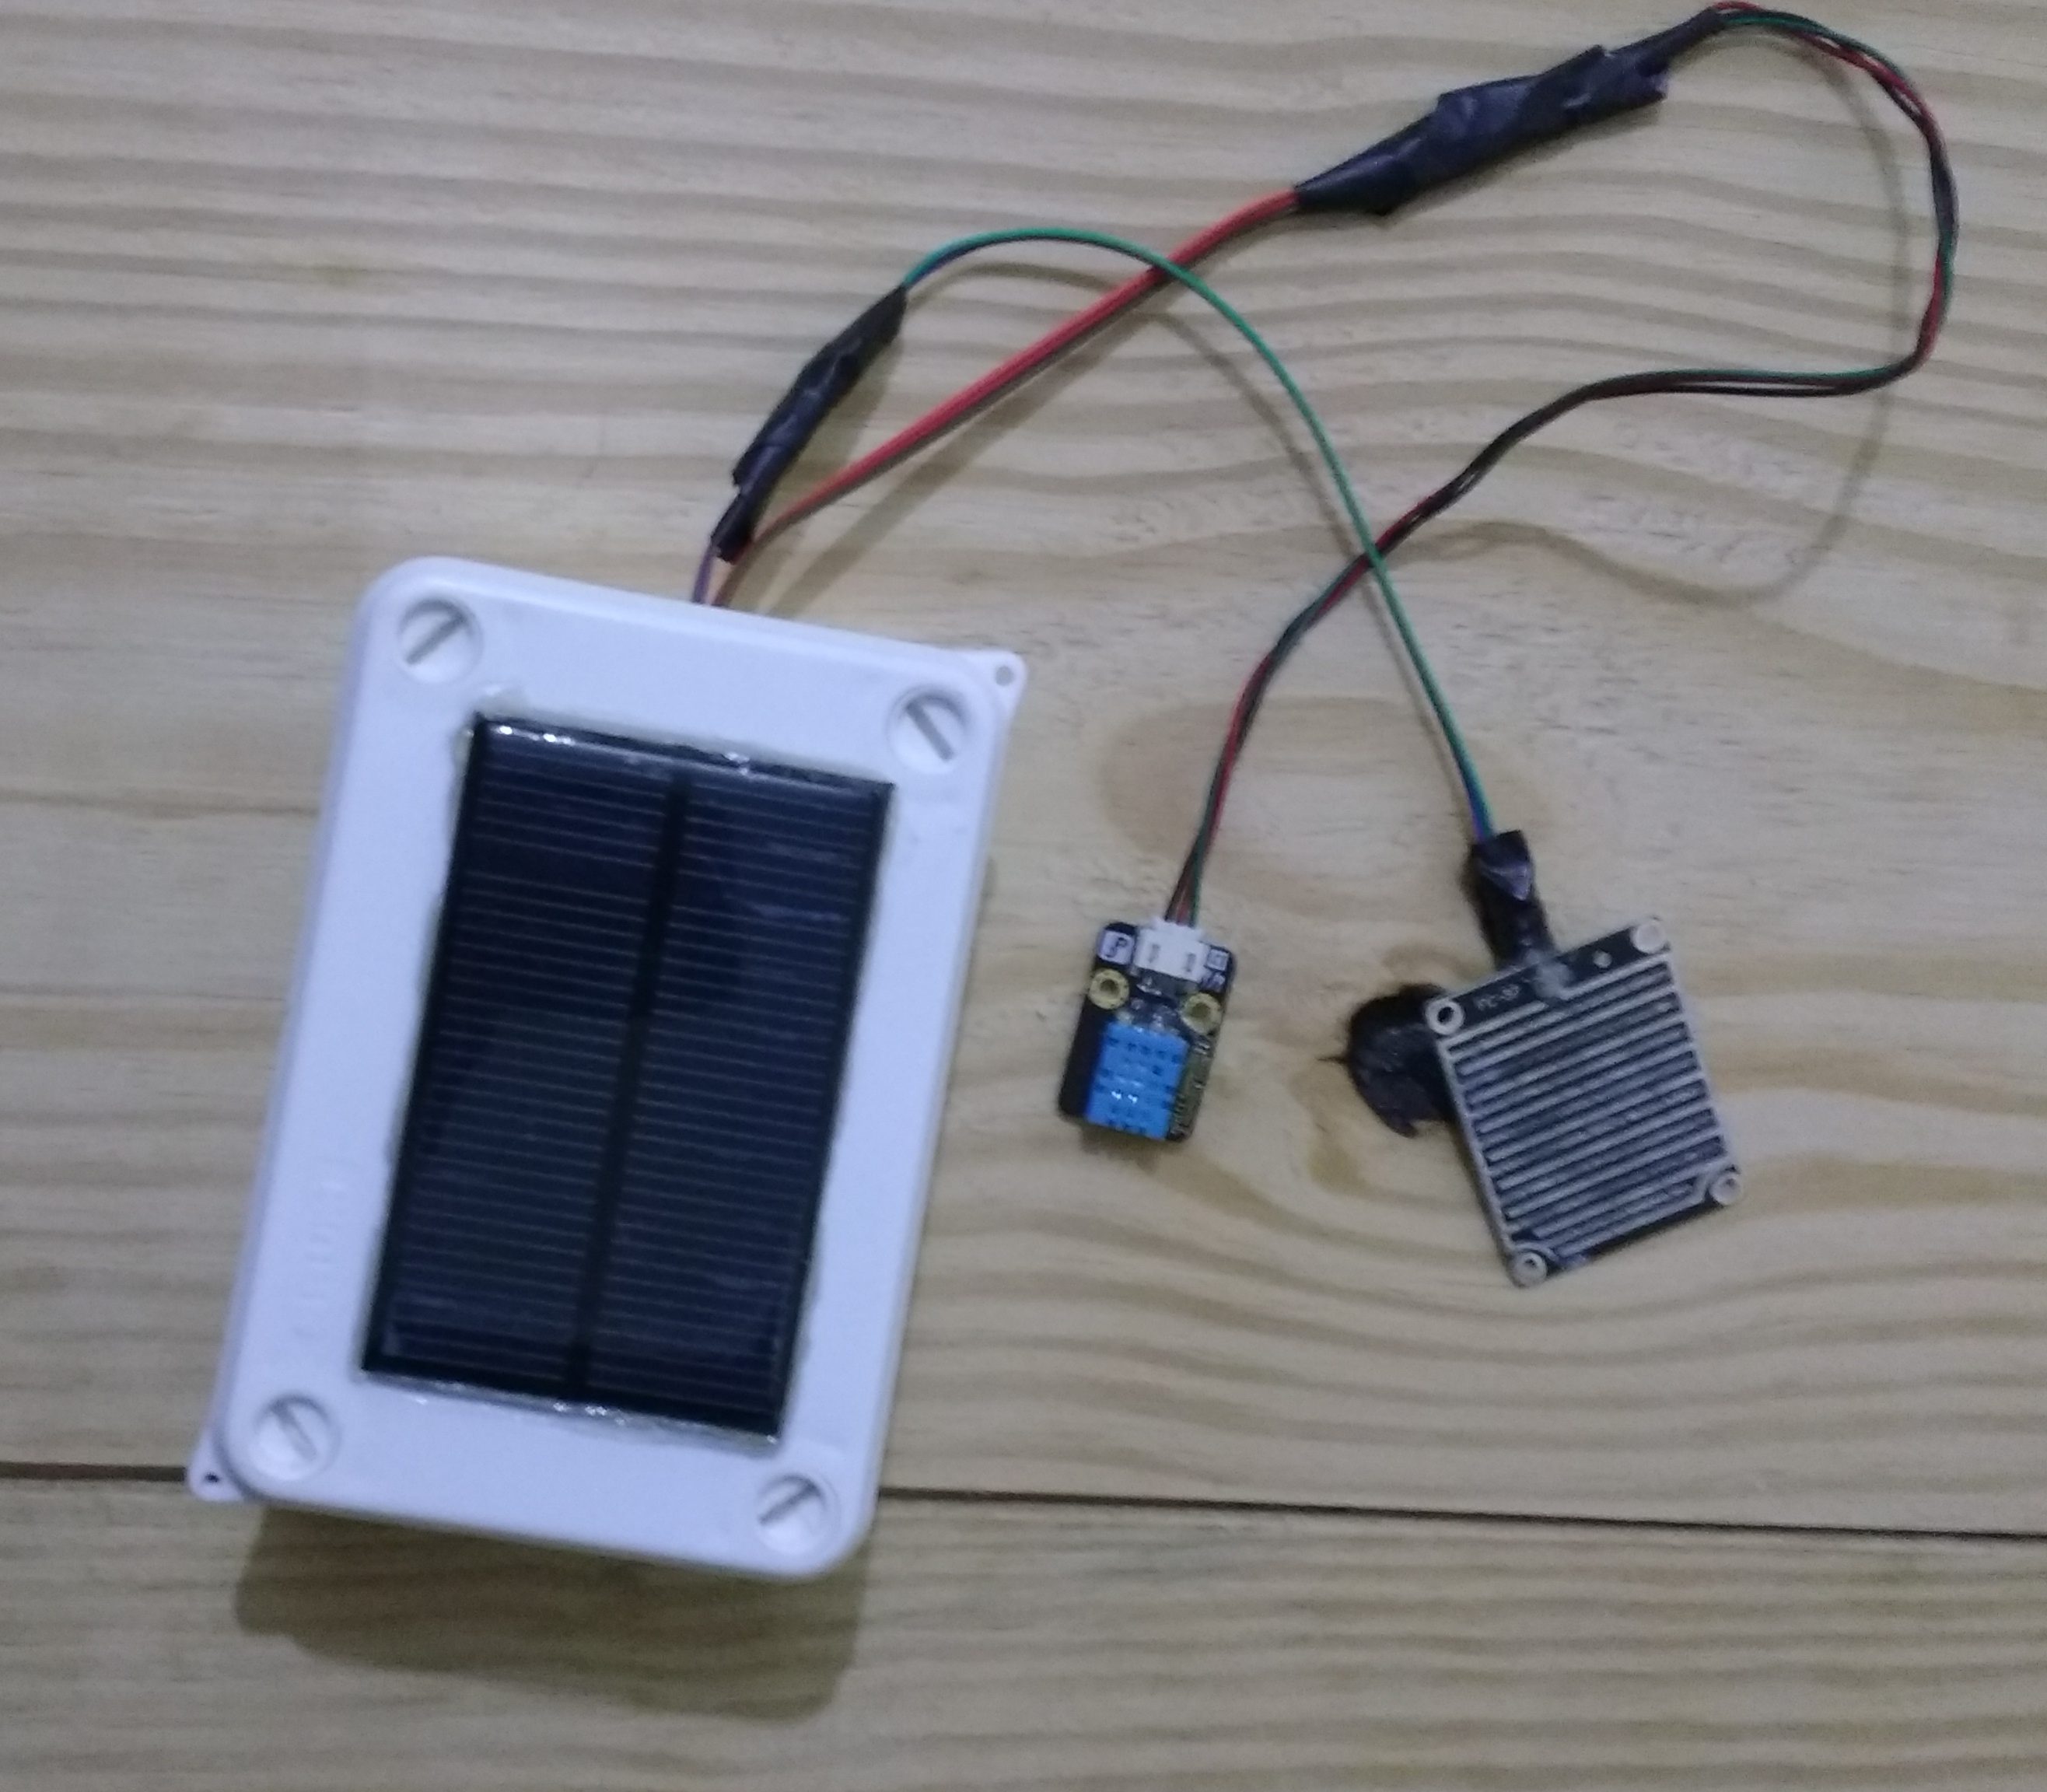
\includegraphics[scale=0.13]{04-figuras/no-exterior2.png}
    \caption{Nó encapsulado pronto para ser instalado.}
    \vspace{-\baselineskip}
    \fonte{Do Autor (2018).}
    \label{fig:no-externo2}
\end{figure}

\section{Aplicação Web}
Nesta seção serão apresentados os resultados parciais obtidos quanto ao desenvolvimento da aplicação web, seguindo os passos listados na Metodologia, seção 4.

\subsection{Levantamento e Análise de Requisitos}
Foram levantados os requisitos que atendem às necessidades do setor. Feito este levantamento, foi definido um escopo para se dar inicio ao desenvolvimento, foi definido que as funcionalidades a serem implementadas serão: 

\begin{itemize}[itemsep=0em]
\item Manter usuários
\item Manter experimentos
\item Manter medições
\item Consultar relatórios
\end{itemize}

\subsection{Projeto de \textit{software}}
A figura \ref{fig:caso-de-uso} mostra o diagrama de caso de uso elaborados de acordo com os requisitos levantados na etapa anterior.

\subsection{Implementação e Implantação}
A figura \ref{fig:tela-login} mostra a tela de autenticação, que é necessário ser efetuado para que o usuário tenha acesso às funcionalidades do sistema. A figura \ref{fig:tela-dashboard} mostra o \textit{dashboard} do sistema, nele são listados as últimas 60 medições realizadas pela rede. À medida que as medições são salvas no banco de dados os gráficos do \textit{dashboard} são atualizados.

\begin{figure}[H]
    \centering
    \includegraphics[scale=0.3]{04-figuras/tela_login.jpg}
    \caption{Tela de \textit{login} do sistema.}
    \vspace{-\baselineskip}
    \fonte{Do Autor (2018).}
    \label{fig:tela-login}
\end{figure}

\begin{figure}[H]
    \centering
    \includegraphics[scale=0.3]{04-figuras/tela_painel.png}
    \caption{Painel do sistema.}
    \vspace{-\baselineskip}
    \fonte{Do Autor (2018).}
    \label{fig:tela-dashboard}
\end{figure}

A figura \ref{fig:tela-listar-usuarios} mostra a tela onde é possível fazer a listagem dos usuários cadastrados no sistema, tendo também as ações de cadastrar ou excluir algum usuário listado. Já na figura \ref{fig:tela-cadastrar-usuario} temos o formulário utilizado para cadastrar um novo usuário e também atualizar as informações de um usuário já existente.

\begin{figure}[H]
    \centering
    \includegraphics[scale=0.3]{04-figuras/tela_listar_usuarios.png}
    \caption{Tela de listar usuários.}
    \vspace{-\baselineskip}
    \fonte{Do Autor (2018).}
    \label{fig:tela-listar-usuarios}
\end{figure}

\begin{figure}[H]
    \centering
    \includegraphics[scale=0.3]{04-figuras/tela_cadastrar_usuario.png}
    \caption{Tela de cadastrar novo usuário.}
    \vspace{-\baselineskip}
    \fonte{Do Autor (2018).}
    \label{fig:tela-cadastrar-usuario}
\end{figure}

A figura \ref{fig:tela-listar-locais} mostra a tela onde é possível fazer a listagem dos locais já cadastrados no sistema, tendo também as ações de cadastrar ou excluir algum local listado. Já na figura \ref{fig:tela-cadastrar-usuario} temos o formulário utilizado para cadastrar um novo local e também atualizar as informações de um local já cadastrado.

\begin{figure}[H]
    \centering
    \includegraphics[scale=0.3]{04-figuras/tela_lista_locais.png}
    \caption{Tela de listar localizações dos nós.}
    \vspace{-\baselineskip}
    \fonte{Do Autor (2018).}
    \label{fig:tela-listar-locais}
\end{figure}

\begin{figure}[H]
    \centering
    \includegraphics[scale=0.3]{04-figuras/tela_cadastra_local.png}
    \caption{Tela de cadastrar novo local.}
    \vspace{-\baselineskip}
    \fonte{Do Autor (2018).}
    \label{fig:tela-cadastrar-local}
\end{figure}

A figura \ref{fig:tela-listar-nos} mostra a tela onde é possível fazer a listagem dos nós já cadastrados no sistema, tendo também as ações de cadastrar ou excluir algum nó listado. Já na figura \ref{fig:tela-cadastrar-no} temos o formulário utilizado para cadastrar um novo nó e também atualizar as informações de um nó já cadastrado.

\begin{figure}[H]
    \centering
    \includegraphics[scale=0.3]{04-figuras/tela_lista_no.png}
    \caption{Tela de listar nós da rede.}
    \vspace{-\baselineskip}
    \fonte{Do Autor (2018).}
    \label{fig:tela-listar-nos}
\end{figure}

\begin{figure}[H]
    \centering
    \includegraphics[scale=0.3]{04-figuras/tela_cadastra_no.png}
    \caption{Tela de cadastrar novo nó.}
    \vspace{-\baselineskip}
    \fonte{Do Autor (2018).}
    \label{fig:tela-cadastrar-no}
\end{figure}


A figura \ref{fig:tela-relatorio-medicoes} mostra a tela onde é emitir um relatório das medições realizadas pela rede em um determinado intervalo de tempo, além de também ter como ação visualizar todas as medições do dia. Já na figura \ref{fig:tela-relatorio-medicoes-dia} temos a listagem de todas as medições realizadas no dia em questão.

\begin{figure}[H]
    \centering
    \includegraphics[scale=0.3]{04-figuras/tela_relatorio_medicoes.png}
    \caption{Tela de medições de um intervalo.}
    \vspace{-\baselineskip}
    \fonte{Do Autor (2018).}
    \label{fig:tela-relatorio-medicoes}
\end{figure}

\begin{figure}[H]
    \centering
    \includegraphics[scale=0.3]{04-figuras/tela_relatorio_medicoes_dia.png}
    \caption{Tela de medições de um dia.}
    \vspace{-\baselineskip}
    \fonte{Do Autor (2018).}
    \label{fig:tela-relatorio-medicoes-dia}
\end{figure}

Na Figura \ref{fig:relatorio-valvulas} é listado, a quantidade de vezes que o sistema nebulizador foi acionado no dia e a duração total em que o nebulizador ficou ativos, dentro de um intervalo informado. Além de ter também a opção de visualizar os acionamentos realizados em um dia específico. A Figura \ref{fig:relatorio-valvulas-detalhes} mostra apenas os acionamentos efetuado em um dia específicos.

\begin{figure}[H]
    \centering
    \includegraphics[scale=0.3]{04-figuras/relatorio-valvulas.png}
    \caption{Tela de acionamentos do nebulizador em um intervalo.}
    \vspace{-\baselineskip}
    \fonte{Do Autor (2018).}
    \label{fig:relatorio-valvulas}
\end{figure}

\begin{figure}[H]
    \centering
    \includegraphics[scale=0.3]{04-figuras/relatorio-valvulas-detalhes.png}
    \caption{Tela de acionamentos do nebulizador em um dia.}
    \vspace{-\baselineskip}
    \fonte{Do Autor (2018).}
    \label{fig:relatorio-valvulas-detalhes}
\end{figure}

\subsection{Implantação do sistema}
Para se dar inicio aos testes do trabalho era necessário um servidor tanto para a aplicação web quanto para o \textit{broker} mqtt. Diante essa demanda foi criado uma conta na Amazon Web Services (AWS)\footnote[8]{Para maiores informações acesse: \url{https://aws.amazon.com/pt/}}, que é uma plataforma de serviços de computação em nuvem.

Com uma maquina virtual Linux disponibilizada pela AWS foi possível fazer a configuração de um servidor web com o Nginx\footnote[9]{Para maiores informações acesse: \url{https://www.nginx.com/}}
e também a configuração do \textit{broker} mqtt Mosquitto. Após concluir as configurações foi realizado o \textit{deploy} da aplicação, tanto backend quanto frontend, para o servidor\footnote[10]{A aplicação pode ser acessada em: \url{https://fruticultura.jonathanfsilva.me}}.

Com a aplicação em funcionamento, foi possível fazer a instalação dos nós dentro da estufa. A Figura \ref{fig:no-publicador-estufa} mostra um nó já instalado na estufa, fazendo a coleta dos valores de temperatura, umidade e molhamento foliar.

\begin{figure}[H]
    \centering
    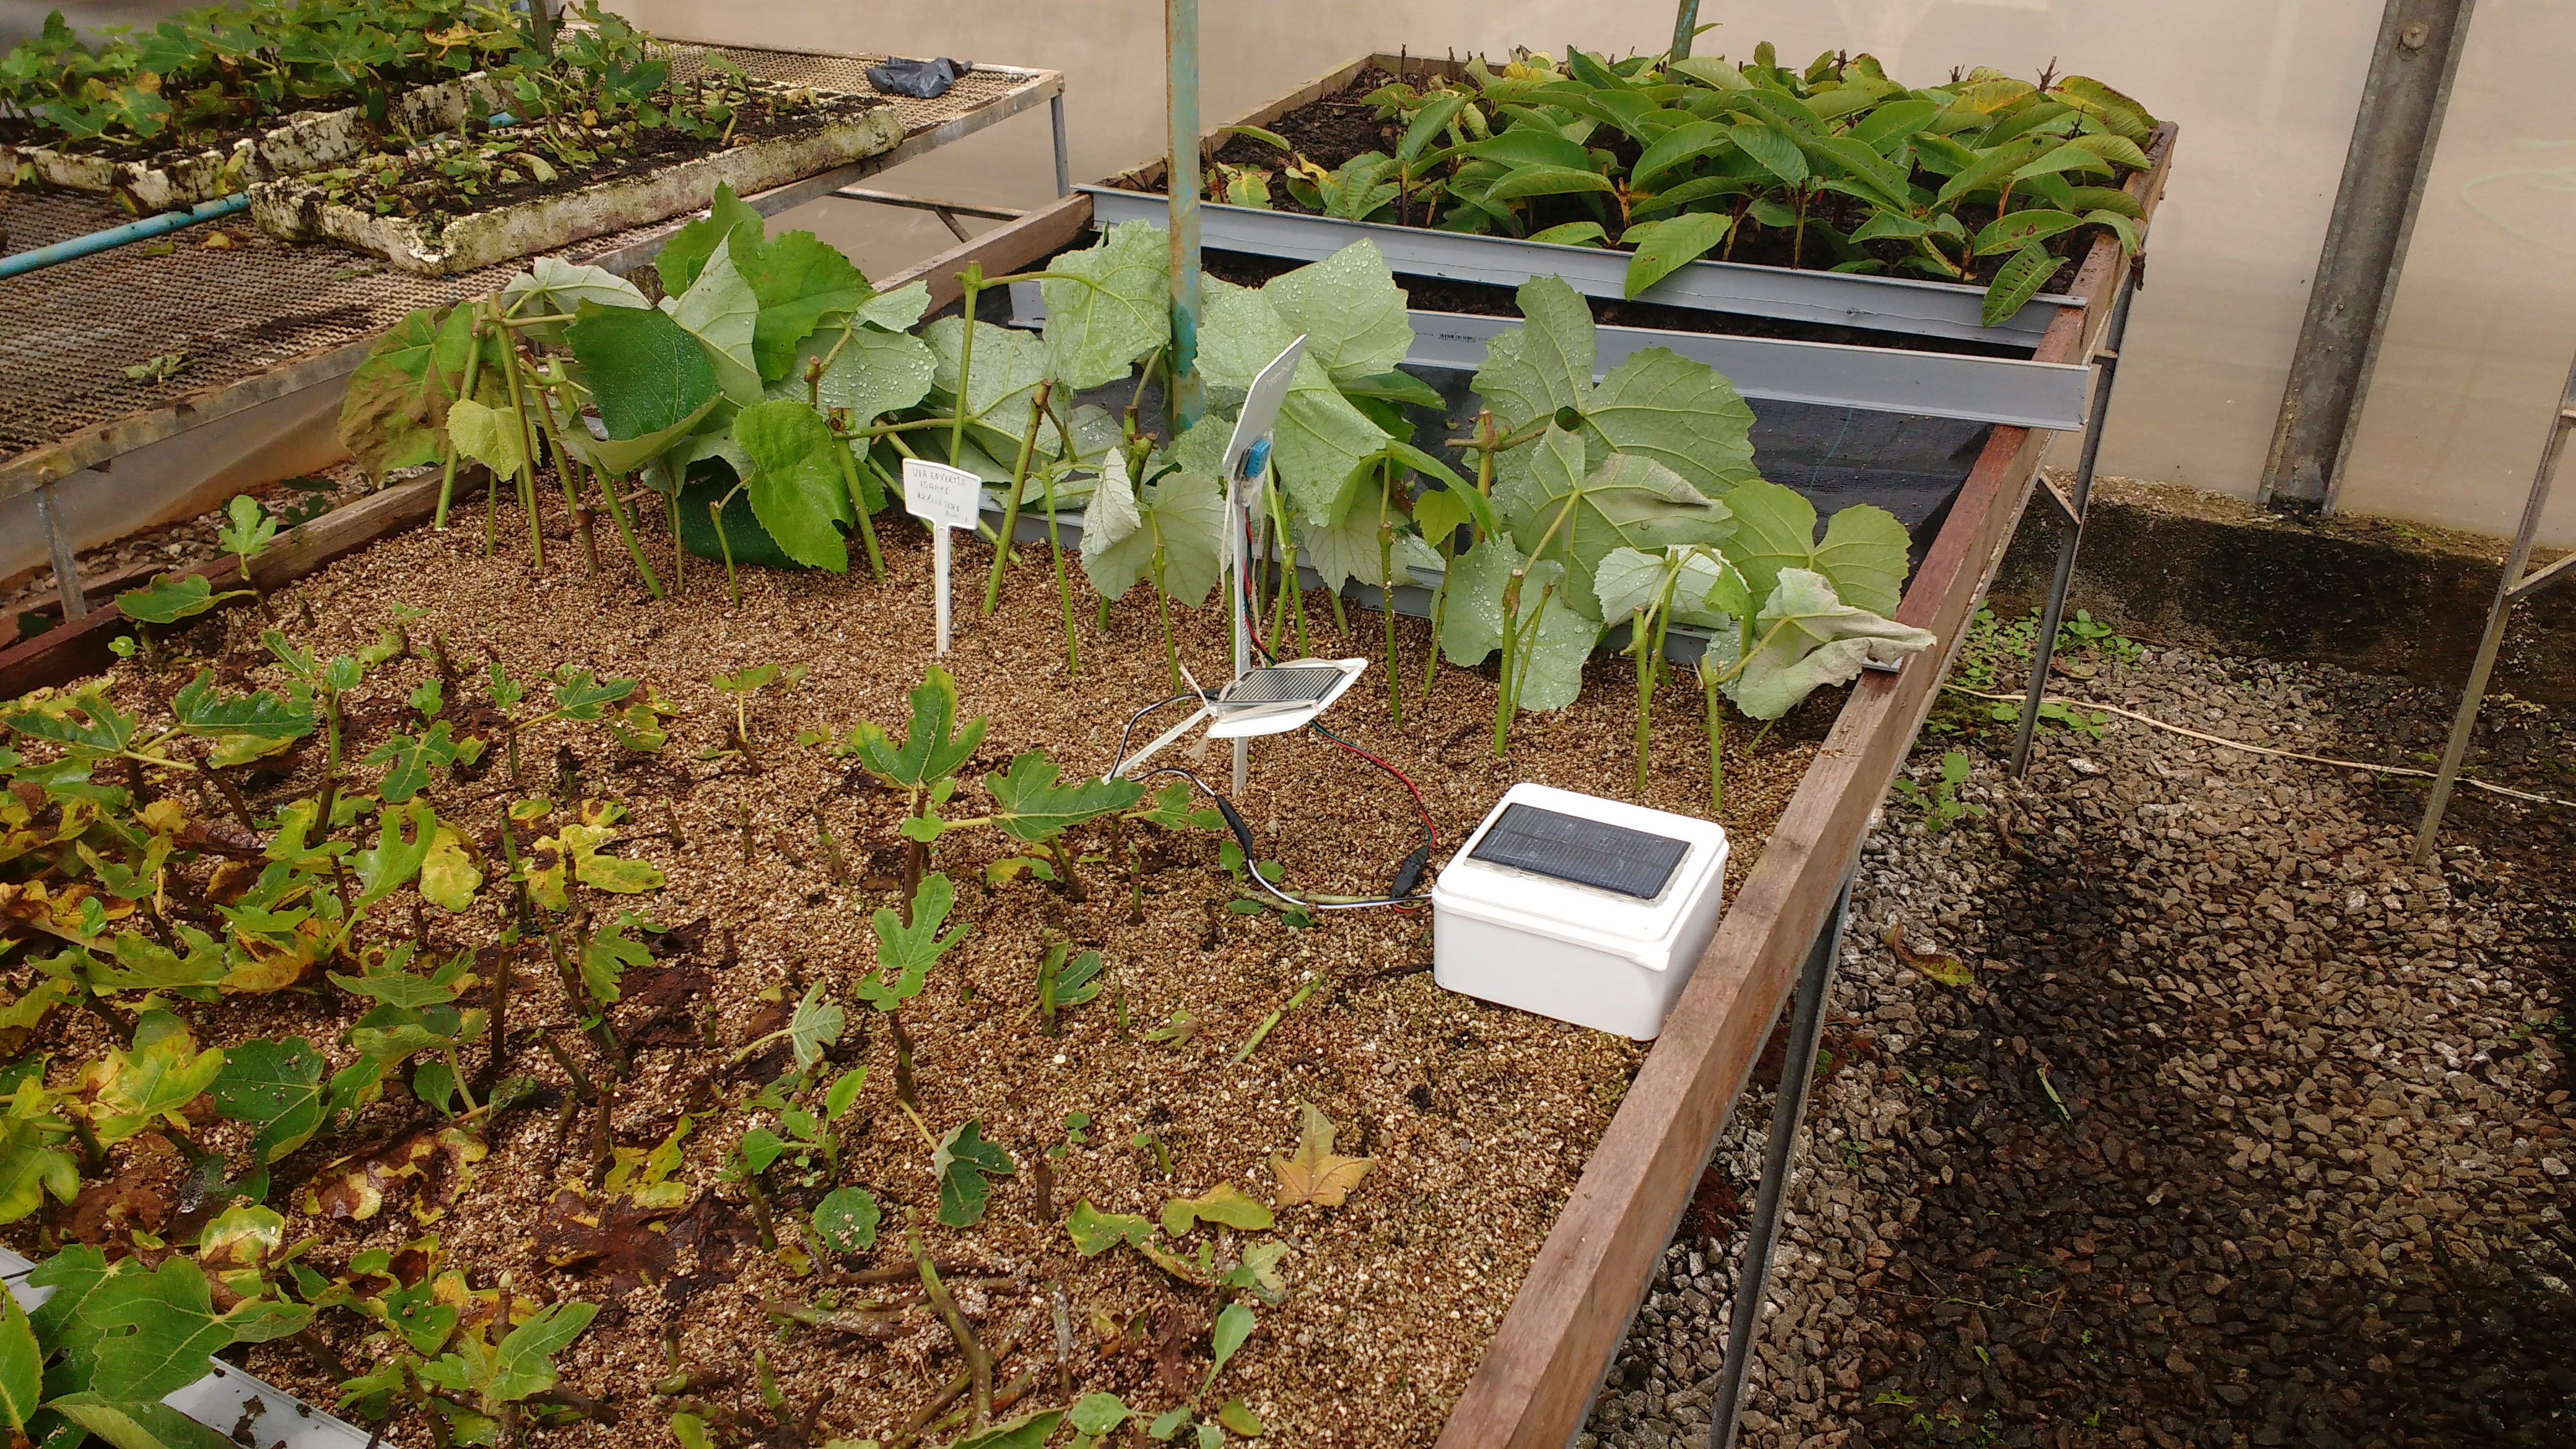
\includegraphics[scale=0.1]{04-figuras/publicador-estufa.jpg}
    \caption{Nó publicador já instalado na estufa.}
    \vspace{-\baselineskip}
    \fonte{Do Autor (2018).}
    \label{fig:no-publicador-estufa}
\end{figure}